\clearpage
% Literaturverzeichnis
%\bibliographystyle{dbstmpl}    % verwendet dbstmpl.bst
%\bibliographystyle{alpha}
%\bibliographystyle{agsm} % probleme mit _ bei urls
\bibliographystyle{plainnat}
\bibliography{dbstmpl}          % verwendet dbstmpl.bib


\appendix
\chapter{Benchmark Dataset Examples}\label{ch:app-datasets}
Figure~\ref{fig:dataset-examples} shows representational examples taken out of benchmark datasets
for \ac{STD}, \ac{STR} and \ac{STS}.
\begin{figure}[hb]
    \centering\scriptsize
    \subfigure[\scriptsize ICDAR (2013) \citep{karatzas_icdar_2013}\label{fig:ICDAR-2013}]
        {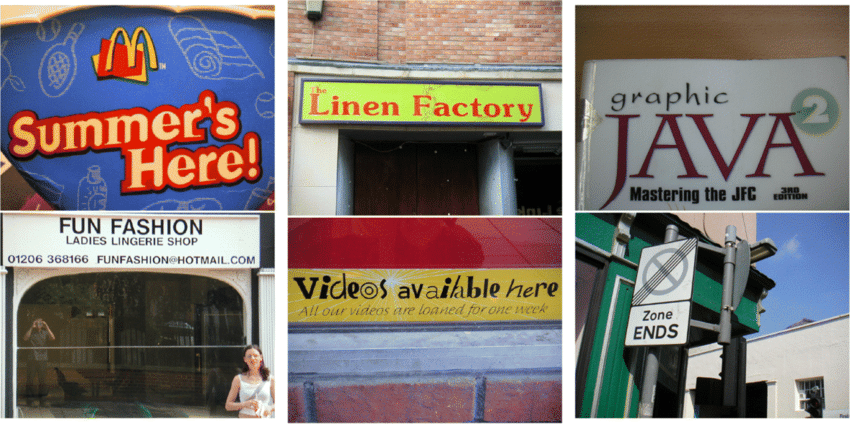
\includegraphics[width=0.20\textwidth]{img/Dataset-Examples/icdar-2013-examples.png}}
    \subfigure[\scriptsize ICDAR (2015) \citep{karatzas_icdar_2015}\label{fig:ICDAR-2015}]
        {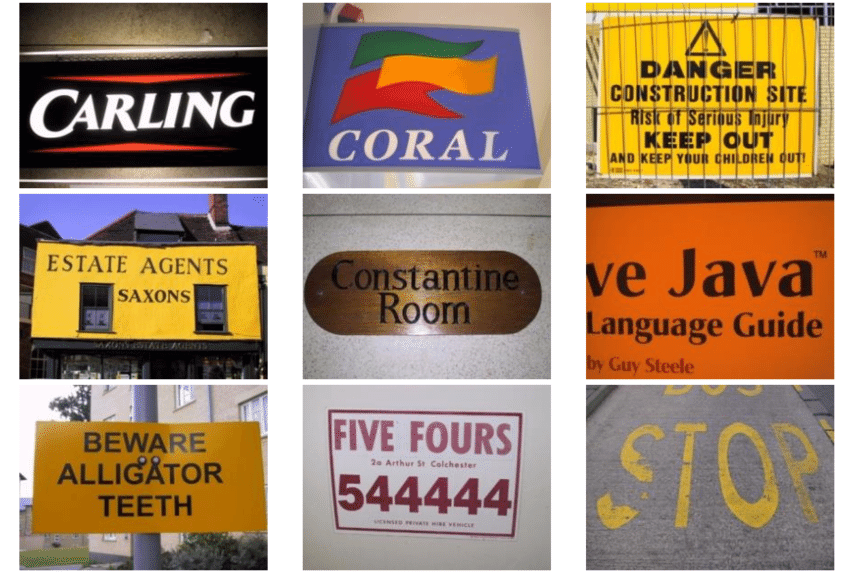
\includegraphics[width=0.25\textwidth]{img/Dataset-Examples/icdar-2015-examples.png}}
    \subfigure[\scriptsize ICDAR MLT (2017) \citep{nayef_icdar2017_2017}\label{fig:ICDAR-2017}]
        {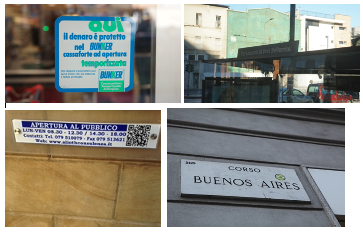
\includegraphics[width=0.20\textwidth]{img/Dataset-Examples/icdar-mlt-2017-examples.png}}
    \subfigure[\scriptsize IIIT 5k Word (2012) \citep{mishra_scene_2012}\label{fig:IIIT-5k}]
        {
\includegraphics[width=0.20\textwidth]{img/Dataset-Examples/IIIT-5k-word-examples.png}}
    \subfigure[\scriptsize MSRA-TD500 \citep{cong_yao_detecting_2012}\label{fig:msra-td500}]
        {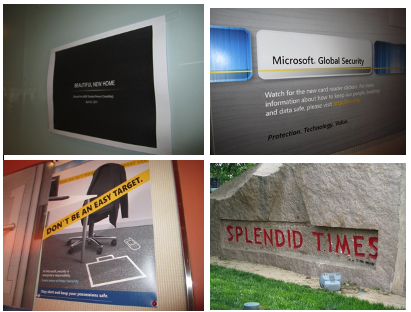
\includegraphics[width=0.20\textwidth]{img/Dataset-Examples/MSRA-TD500-examples.png}}
    \subfigure[\scriptsize Total Text (2017) \citep{chng_total-text_2017}\label{fig:total-text}]
        {
\includegraphics[width=0.20\textwidth]{img/Dataset-Examples/Total-Text-examples.png}}
    \subfigure[\scriptsize SCUT CTW1500 (2017) \citep{yuliang_detecting_2017}\label{fig:SCUT-CWT1500}]
        {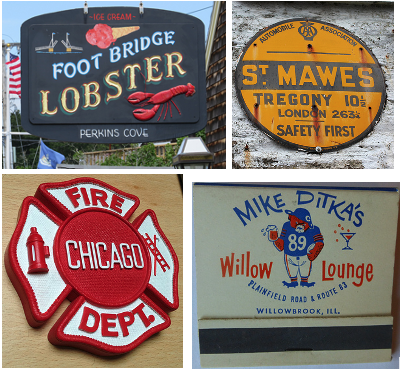
\includegraphics[width=0.20\textwidth]{img/Dataset-Examples/SCUT-CWT1500-examples.png}}
    \caption{Benchmark Data Set Examples\label{fig:dataset-examples}}
\end{figure}

\chapter{Litaratur Qualities}

% FIXME: for table: zurodnung zum Teil selber vorgenommen
The following tables show qualities that where identified in literature.
The qualities are categorized by the \ac{MLS} entities defined in~\cite{siebert_construction_2021}.
The model entity is the focus of this work and is thus discussed in Chapter~\ref{ch:problem}.
\begin{table}[h]\label{tb:LiteratureQualitiesData}
    \centering\footnotesize
    \begin{tabular}{p{.4\textwidth} p{.5\textwidth}}
        \textbf{Qualitiy} & \textbf{Sources} \\
        \toprule
        Relevancy &~\cite{ashmore_assuring_2021} \\
        Currentness &~\cite{siebert_construction_2021} \\
        Completeness &~\cite{ashmore_assuring_2021, vogelsang_requirements_2019,
                            siebert_construction_2021} \\
        Balancedness &~\cite{ashmore_assuring_2021,siebert_construction_2021} \\
        Consistency &~\cite{vogelsang_requirements_2019} \\
        Intra-Consistency &~\cite{siebert_construction_2021} \\
        Inter-Consistency &~\cite{siebert_construction_2021} \\
        Accuracy &~\cite{ashmore_assuring_2021} \\
        Absence of bias &~\cite{siebert_construction_2021} \\
        Correctness &~\cite{vogelsang_requirements_2019} \\
        Data Representativeness&~\cite{nakamichi_requirements-driven_2020,
                                    siebert_construction_2021}\\
        Suitability of Training Data &~\cite{nakamichi_requirements-driven_2020} \\
        Test Dataset Creating Appropriateness &~\cite{nakamichi_requirements-driven_2020} \\
        Independence of Train and Test Data &~\cite{nakamichi_requirements-driven_2020,
                                                    siebert_construction_2021} \\
    \end{tabular}
    \caption{MLS qualities identified for data entity}
\end{table}

\begin{table}[h]\label{tb:LiteratureQualitiesInfrastructure}
    \centering\footnotesize
    \begin{tabular}{p{.4\textwidth} p{.5\textwidth}}
        \textbf{Qualitiy} & \textbf{Sources} \\
        \toprule
        Capacity of Data Storage &~\cite{nakamichi_requirements-driven_2020} \\
        Infrastructure suitability &~\cite{siebert_construction_2021} \\
        Deployment Fit-for-Purpose &~\cite{ashmore_assuring_2021} \\
        Training Process Appropriateness &~\cite{nakamichi_requirements-driven_2020} \\
        Training efficiency &~\cite{siebert_construction_2021} \\
    \end{tabular}
    \caption{MLS qualities identified for infrastrucure entity}
\end{table}

\begin{table}[h]\label{tb:LiteratureQualitiesEnvironment}
    \centering\footnotesize
    \begin{tabular}{p{.4\textwidth} p{.5\textwidth}}
        \textbf{Qualitiy} & \textbf{Sources} \\
        \toprule
        Coverage of Usage Environment &~\cite{nakamichi_requirements-driven_2020} \\
        Coverage of Operation Environment &~\cite{nakamichi_requirements-driven_2020} \\
        Scope compliance &~\cite{siebert_construction_2021} \\
        Social impact &~\cite{siebert_construction_2021} \\
        Environmental Impact of training process &~\cite{siebert_construction_2021}\\
        Contextual Relevancy &~\cite{ashmore_assuring_2021} \\
    \end{tabular}
    \caption{MLS qualities identified for environment entity}
\end{table}

\begin{table}[h]\label{tb:LiteratureQualitiesSystem}
    \centering\footnotesize
    \begin{tabular}{p{.4\textwidth} p{.5\textwidth}}
        \textbf{Qualitiy} & \textbf{Sources} \\
        \toprule
        Suitability of Input Data Quality Maintenance &~\cite{nakamichi_requirements-driven_2020} \\
        Quality Maintenance for Test Data Appropriateness&~\cite{nakamichi_requirements-driven_2020}\\
        Security and Privacy Assurance&~\cite{nakamichi_requirements-driven_2020,zhang_machine_2020}\\
        Troubleshooting &~\cite{arpteg_software_2018} \\
        Easiness of Resource Update &~\cite{nakamichi_requirements-driven_2020} \\
        Easiness of Software Update &~\cite{nakamichi_requirements-driven_2020} \\
        Easiness of System Status Analysis &~\cite{nakamichi_requirements-driven_2020} \\
        Runtime correctness &~\cite{siebert_construction_2021} \\
        Legal and Regularity Requirements &~\cite{vogelsang_requirements_2019} \\
        Effectiveness of output supervision &~\cite{siebert_construction_2021} \\
        Efficiency of output supervision &~\cite{siebert_construction_2021} \\
        Appropriateness of Operation Maintenance &~\cite{nakamichi_requirements-driven_2020} \\
        Deployment Tolerability &~\cite{ashmore_assuring_2021} \\
        Deployment Adaptability &~\cite{ashmore_assuring_2021} \\
    \end{tabular}
    \caption{MLS qualities identified for system entity}
\end{table}
